%%%%%%%%%%%%%%%%%%%%%%%%%%%%%%%%%%%%%%%%%%%%%%%%%%%%%%%%%%%%%%%%%%%%%%%%%%%
%                                                                         %
%			TEMPLATE LATEX PER TESI                                       %
%			______________                                                %
%                                                                         %
%           Ultima revisione: 24 giugno 2019                              %
%           Revisori: G.Presti; L.A.Ludovico; F. Avanzini                 %
%                                                                         %
%%%%%%%%%%%%%%%%%%%%%%%%%%%%%%%%%%%%%%%%%%%%%%%%%%%%%%%%%%%%%%%%%%%%%%%%%%%

\documentclass[12pt,italian]{report}
\usepackage{tesi}

%
%			INFORMAZIONI SULLA TESI
%			DA COMPILARE!
%

% CORSO DI LAUREA:
\def\myCDL{Corso di Laurea triennale in\\Informatica}

% TITOLO TESI:
\def\myTitle{Riconoscimento di volti tramite insiemi fuzzy}

% AUTORE:
\def\myName{Tommaso Amadori}
\def\myMat{Matr. Nr. 892859}

% RELATORE E CORRELATORE:
\def\myRefereeA{Prof. Dario Malchiodi}
\def\myRefereeB{Prof. Anna Maria Zanaboni}

% ANNO ACCADEMICO
\def\myYY{2018-2019}

% Il seguente comando introduce un elenco delle figure dopo l'indice (facoltativo)
%\figurespagetrue

% Il seguente comando introduce un elenco delle tabelle dopo l'indice (facoltativo)
%\tablespagetrue

%
%			PREAMBOLO
%			Inserire qui eventuali package da includere o definizioni di comandi personalizzati
%

% Package di formato
\usepackage[a4paper]{geometry}		% Formato del foglio
\usepackage[italian]{babel}			% Supporto per l'italiano
\usepackage[utf8]{inputenc}			% Supporto per UTF-8
%\usepackage[a-1b]{pdfx}			% File conforme allo standard PDF-A (obbligatorio per la consegna)

% Package per la grafica
\usepackage{graphicx}				% Funzioni avanzate per le immagini
\usepackage{hologo}					% Bibtex logo with \hologo{BibTeX}
%\usepackage{epsfig}				% Permette immagini in EPS
%\usepackage{xcolor}				% Gestione avanzata dei colori

% Package tipografici
\usepackage{amssymb,amsmath,amsthm} % Simboli matematici
\usepackage{listings}				% Scrittura di codice

% Package ipertesto
\usepackage{url}					% Visualizza e rendere interattii gli URL
\usepackage{hyperref}				% Rende interattivi i collegamenti interni
\usepackage{algorithm}
\usepackage[noend]{algpseudocode}
\usepackage{amsmath}
\usepackage{amsfonts}
\usepackage{verbatimbox}

\setcounter{secnumdepth}{3}
\setcounter{tocdepth}{3}
\begin{document}

% Creazione automatica del frontespizio
\frontespizio
\beforepreface

% 
%			PAGINA DI DEDICA E/O CITAZIONE
%			facoltativa, questa è l'unica cosa che dovete formattare a mano, un po' come vi pare
%

         
% 
%			PREFAZIONE (facoltativa)
%

%\prefacesection{Prefazione}
%Le prefazioni non sono molto comuni, tuttavia a volte capita che qualcuno voglia dire qualcosa che esuli dal lavoro in s\'e (come un meta-commento sull'elaborato), o voglia fornire informazioni riguardanti l'eventuale progetto entro cui la tesi si colloca (in questo caso \`e probabile che sia il relatore a scrivere questa parte).

%
%			RINGRAZIAMENTI (facoltativi)
%


%
%			Creazione automatica dell'indice
%

\afterpreface

% 
%			CAPITOLO 1: Introduzione o Abstract
% 

\chapter{Apprendimento automatico}
\label{cap:apprendimento_automatico}
Il Machine Learning insegna ai computer a compiere attività in modo naturale come gli esseri umani o gli animali: imparando dall’esperienza. In sostanza, gli algoritmi di Machine Learning usano metodi matematico-computazionali per apprendere informazioni direttamente dai dati, senza modelli matematici ed equazioni predeterminate. Gli algoritmi di Machine Learning migliorano le loro prestazioni in modo “adattivo” mano a mano che gli “esempi” da cui apprendere aumentano. Cerchiamo allora di capire cos’è il Machine Learning, come funziona e quali sono le sue applicazioni.
\section{Approcci}
\label{sec:approcci}

I tipi di algoritmi di machine learning differiscono nel loro approccio, nel tipo di dati che utilizzano, producono e nel tipo di attività o problema che devono risolvere. Il machine learning può generalmente essere suddiviso in tre macro categorie: 
\begin{itemize}
	\item supervisionato
	\item non supervisionato
	\item apprendimento con rinforzo
\end{itemize}
A queste viene aggiunta anche una quarta che si chiama "semi-supervisionato".


\subsection{Supervisionato}

L'approccio supervisionato è una tecnica che prevede di lavorare su un insieme di dati etichetti dall'utente, da cui possa imparare a riconoscerne le varie differenze e in seguito a fare una predizione sulla possibile classificazione. Questa tecnica può fornire due diversi tipi di risultati: discreti o continui. Per comprendere meglio questo concetto proviamo a fare un esempio.

Prendiamo delle diagnosi mediche fatte su una serie di pazienti. Analizzando le diagnosi, un medico è in grado di definire se il paziente è in salute o meno. Da qui possiamo estrapolare quindi due insiemi/etichette differenti per il nostro caso: "in salute" e "malato". Fornendo come input ad un classificatore questo insieme di dati con le rispettive etichette appena definite, il calcolatore, tramite un'algoritmo supervisionato, sarà in grado di fornire delle predizioni sulla possibile etichetta da attribuire ad ogni nuova diagnosi.

È importante che l'input, sia consistente. In altre parole, è importante che vi siano molti dati da analizzare, perché può capitare, che se questi sono pochi, la capacità di predizione dell'algoritmo sarà di scarsa qualità.

In questo esempio abbiamo utilizzato solamente le classi "in salute" e "malato", ma nulla ci vieta di definirne una terza o una quarta, ad esempio possiamo etichettare un paziente come "asmatico" o "diabetico".\\


Nel caso in cui, non vogliamo avere solo una classificazione della salute del paziente, ma preferiamo quantificare l'aspettativa di vita, non è più possibile ricorrere a dei classificatori. Da qui nasce la necessità di passare da un valore discreto ad un valore continuo: i regressori. 

I regressori servono nel momento in cui si vuole quantificare una caratteristica che descrive un oggetto. Ad esempio, potremmo voler quantificare i tempi di guarigione per un paziente malato, data una specifica diagnosi.

I modelli di machine learning supervisionati hanno l'obiettivo di fare con la maggior precisione possibile, una predizione su dati nuovi, mai visti prima. Per raggiungere questo scopo dobbiamo assicurarci che il modello stia lontano dal sovra-adattamento (overfitting) e del sotto-adattamento (underfitting). Vediamoli in dettaglio.
L'overfitting si verifica quando il modello tende ad adattarsi in maniera eccessiva ai dati che gli sono stati forniti per allenarsi, il che non permette di generalizzare bene il modello per nuovi dati. Questo perché anche con un piccolo scostamento dai vincoli che determinano la predizione, comporterebbe una predizione sbagliata.
L'underfitting invece, si verifica nel caso contrario dell'overfitting. Esso definisce la situazione in cui il modello si basa su delle regole troppo semplici e poco robuste, il che comporta la definizione di regole con scarsa qualità su come si riconosca un oggetto.

\begin{table}[h!]
	\center
	\caption{Dati di esempio riguardo clienti}
	\label{table_customers}
	\vspace{3 mm}
	\begin{tabular}{|c|c|c|c|c|c|}
		\hline
		Età & Macchine &  Case possedute & Figli & Stato civile & Barca    \\
		\hline
		66 & 1 & Sì & 2 & Vedova & Sì \\
		52 & 2 & Sì & 3 & Sposato & Sì \\
		22 & 0 & No & 0 & Sposato & No \\
		25 & 1 & No & 1 & Single & No \\
		44 & 0 & No & 2 & Divorziato & No \\
		39 & 1 & Sì & 2 & Sposato & No \\
		26 & 1 & No & 2 & Single & No \\
		40 & 3 & Sì & 1 & Sposato & No \\
		53 & 2 & Sì & 2 & Divorziato & Sì \\
		64 & 2 & Sì & 3 & Divorziato & No \\
		58 & 2 & Sì & 2 & Sposato & Sì \\
		33 & 1 & No & 1 & Single & No \\
		\hline
	\end{tabular}
\end{table}

Per un esempio più concreto, prendiamo spunto da un esempio riportato nel libro "Introduction to Machine Learning with Python". Basandoci sulla tabella \ref{table_customers} vediamo quali siano i problemi generabili dall'overfitting e dall'underfitting. Supponiamo di voler predire se il cliente X vorrà acquistare una barca. Analizzando la tabella piuttosto attentamente si può notare che secondo la regola: "Se un cliente ha più di 45 anni, ha meno di 3 figli o non è divorziato, allora lui vorrà comprare una barca", secondo la quale, le predizioni (su questo dataset) saranno giuste al 100\%! 

Ma questo significherebbe anche, che se in futuro un cliente C che volesse comprare la barca non rispettasse la regola (magari perché ha semplicemente 44 anni o perchè ha 4 figli), la predizione del sistema sarebbe "C non vuole comprare una barca", quindi errata. Questo è il caso dell'overfitting: stabilire le regole di predizione su troppi dati, in maniera troppo rigida.

Lo stesso si può fare al contrario, ossia quando le regole di predizione adottate dal modello si basano su troppi pochi dati e/o sono troppo vaghe. Supponiamo che il sistema identifichi un cliente come possibile acquirente di una barca se segue la seguente regola: "Se un cliente ha una casa allora vorrà comprare una barca" è naturale, leggendo la regola, pensare che questa sia sbagliata. Questo è il caso dell'underfitting, ossia il caso in cui si definisce un modello che segue regole che generalizzano in maniera eccessiva la regola per che consente di determinarne la classe.

Quindi quello che vogliamo trovare è un modello che sia a metà tra l'overfitting e l'underiffing.
In figura \ref{fig:tradeoff_img} è mostrato un grafico dove lo \textit{sweetspot} identifica un modello ottimale. 

\begin{figure} [h!]


	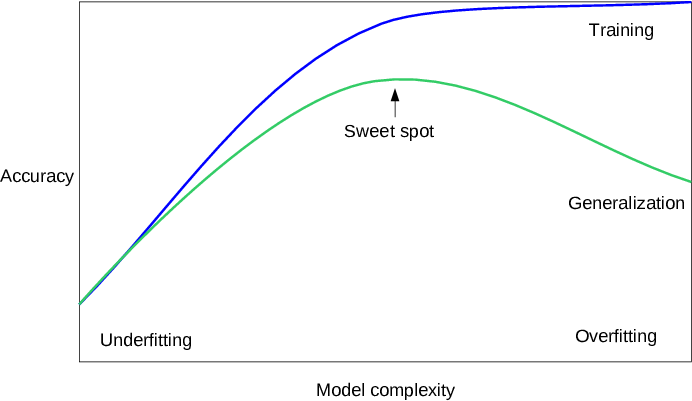
\includegraphics[scale=0.5]{../img/tradeoff_overfitting_underfitting.png}
	\caption{Trade-off tra overfitting e underfitting}
	\label{fig:tradeoff_img}
\end{figure}

% TODO: dal libro
\pagebreak

\subsubsection{k-Nearest Neighbor}

Vediamo nello specifico uno dei più semplici algoritmi di machine learning: k-Nearest Neighbor. Questo è un algoritmo utilizzato sia per la classificazione che per la regressione. In entrambi i casi l'algoritmo si basa sul un parametro k fissato. Questo k definisce il numero di vicini da prendere in considerazione per fare la predizione. Vediamo come si comporta nel dettaglio.

\vspace{5 mm}
\begin{figure}[h!]
	\center
	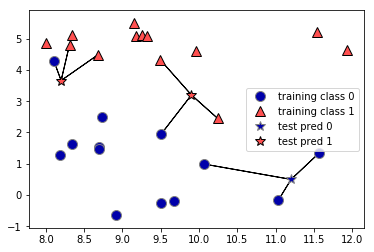
\includegraphics[scale=0.7]{../img/knn_classifier}
	\caption{k-NN classifier}
	\label{fig:knn_classifier}
\end{figure}

Supponiamo di avere due caratteristiche (per semplicità), $ feature_{0} $ e $ feature_{1} $ le quale descriveranno - insieme all'etichetta - ogni record del nostro dataset. 

Nel caso di classificazione tramite il k-NN, come vediamo in figura \ref{fig:knn_classifier} un nuovo elemento non ancora etichettato, verrà classificato in base al tipo predominante dei suoi vicini. La scelta del k, è quindi l'unica, ma fondamentale, scelta da prendere per determinare la precisione nella predizione dei futuri elementi.


\vspace{5 mm}
\begin{figure}[h!]
	\center
	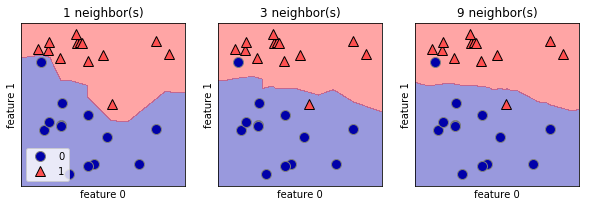
\includegraphics[scale=0.55]{../img/knn_comparison}
	\caption{k-NN classifier con k differenti}
	\label{fig:knn_difference}
\end{figure}


In figura \ref{fig:knn_difference} viene mostrato come influisce la scelta di differenti parametri $ k $ su uno stesso campione.

Questo algoritmo è spesso utilizzato con un $ k $ dispari, il quale non permette di avere casi di indecisione e quindi poter sempre definire la classe del nuovo dato.

Nel caso di regressione tramite il k-NN, il risultato sarà pari alla media del valore target che vogliamo predire di tutti i k vicini. Vediamo un esempio in dettaglio del funzionamento.

\begin{figure}[h!]
	\center
	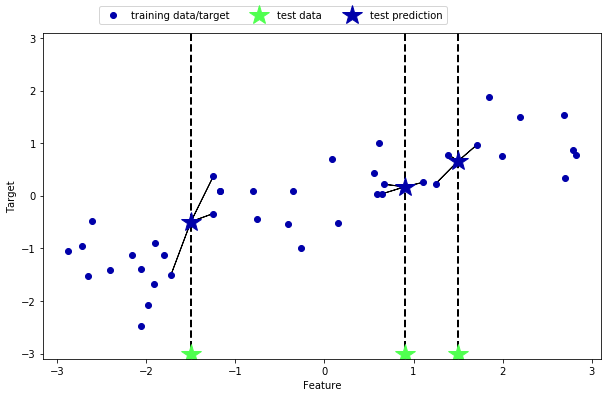
\includegraphics[scale=0.6]{../img/knn_regressor}
	\caption{k-NN regressor}
	\label{fig:knn_regressor}
\end{figure}

Immaginiamo che nel nostro dataset abbiamo due caratteristiche $ feature $ e $target$ per ogni elemento, dove $feature $ è il valore su cui vogliamo basare il modello e $target$ è il valore che siamo interessati a predire. Prendendo ad esempio, un $ k $ pari a 3 significherà (come vediamo in figura \ref{fig:knn_regressor}) che il nuovo elemento (la stella verde) avrà come valore $ target $ (la stella blu) la media dei $ target $ dei 3  elementi più vicini sull'asse delle ascisse (ovvero l'asse su cui sono disposte le $feature$)



\pagebreak
\subsubsection{Linear models}
I modelli lineari sono una classe di modelli che cercano di effettuare predizioni utilizzando una funzione lineare basata sull'insieme delle feature o caratteristiche dell'elemento da analizzare. 
Nel caso della regressione, la funzione di cui parliamo è definibile come segue:
\[ y = w_{0} * x_{0} + w_{1} * x_{1} + ... + w_{n} * x_{n} + b \]


dove $n$ rappresenta il numero di feature, $x$ le feature, $ w $ i pesi da attribuire alle singole feature e la $ b $ rappresenta i parametri attribuiti al modello che si sta allenando.
Prendendo una sola feature (quindi $ n $ pari a 1), $ y $ risulterebbe:

\[ y = w_{0} * x_{0} + b\]

la quale è esattamente una funzione di una linea retta, dove $ w $ è il coefficiente angolare e $ b $ è lo scostamento dall'origine degli assi.

Per riprendere l'esempio precedente, supponiamo che si voglia quantificare il numero di giorni necessari per guarire un paziente malato.
Supponiamo, per semplicità, di avere una sola caratteristica definita all'interno della diagnosi che rappresenta l'età del paziente (sull'asse delle ascisse) e per ogni punto il relativo tempo di guarigione - in giorni - (sull'asse delle ordinate). 
Avendo quindi una serie di punti, è possibile tracciare una retta che approssima a tutti i punti definiti nel campione di allenamento (anche chiamato training set). In figura \ref{fig:linear_regression} è illustrata la retta appena citata.

\begin{figure}[h!]
	\center
	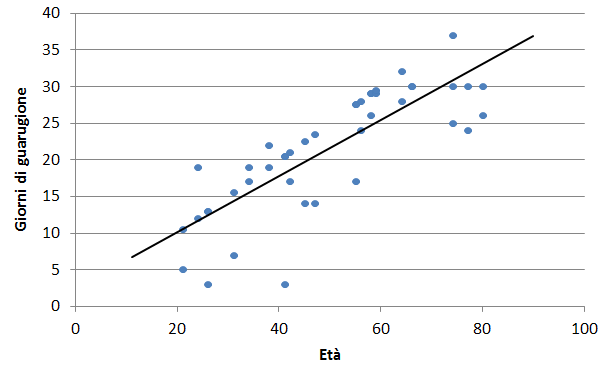
\includegraphics[scale=0.6]{../img/linear_regression}
	\caption{Linear regression}
	\label{fig:linear_regression}
\end{figure}

Tutto questo, per quanto riguarda l'utilizzo di modelli lineari nella regressione. Nella classificazione, invece, si mantiene la stessa formula con una piccola differenza. Si introducono degli intervalli per definire a quale classe appartiene il singolo caso. Nella classificazione binaria, ad esempio la formula risulterebbe come segue:
\[ y = w_{0} * x_{0} + w_{1} * x_{1} + ... + w_{n} * x_{n} + b > 0 \]

dove, supponendo di avere le classi "1" e "0", se la $ y $ fosse maggiore di $ 0 $ appartiene alla classe "1", alla classe "0" altrimenti.
%
%Nella figura xxx è mostrato l'esempio appena citato, dove i cerchi sono la classe 0 e i triangoli la classe 1.

\pagebreak

\subsubsection{Support Vector Machine}
Le SVM (Support Vector Machine) sono una classe di modelli che si preoccupa di individuare un iperpiano utile a separare (e quindi classificare) i punti nel piano in diversi gruppi. 

Il primo problema che le SVM devono risolvere, è capire quale sia l'iperpiano che suddivide nel modo "migliore" i dati. Per capire come l'algoritmo definisca "migliore" un certo sistema di suddivisione, vediamo la figura \ref{fig:svc}.

\begin{figure}[h!]
	\center
	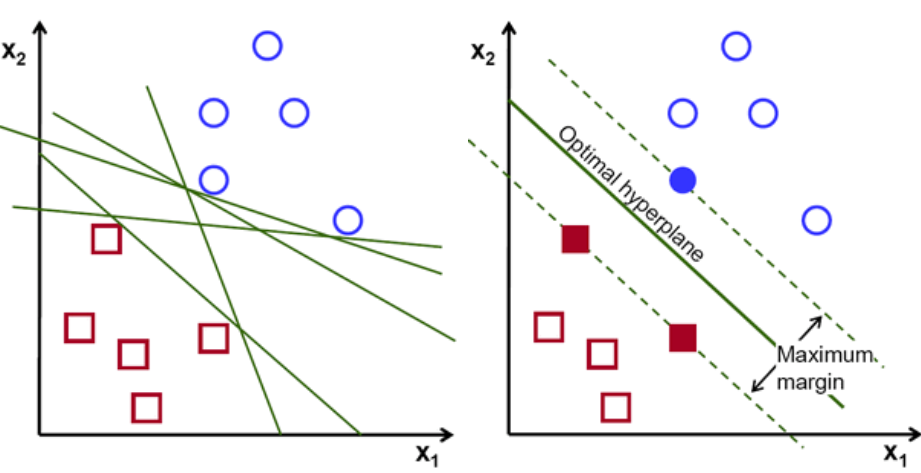
\includegraphics[scale=0.4]{../img/svc} %https://medium.com/@george.drakos62/support-vector-machine-vs-logistic-regression-94cc2975433f
	\caption{Support Vector Machine}
	\label{fig:svc}
\end{figure}

Nella figura di sinstra è possibile notare due gruppi distinti di punti (i cerchi blu e i quadrati rossi), i quali possono essere divisi dagli iperpiani raffigurati in verde. Questi sono i candidati ad essere i "migliori" divisori per i due insiemi.
Una volta presi gli iperpiani candidati, per decidere qual'è il migliore, si prendono i punti P più vicini a questo iperpiano I, i quali vengono definiti vettori di supporto. Per ogni iperpiano I e i relativi vettori di supporto V, viene calcolata la distanza tra I e V la quale indicherà il "margine". Si definisce quindi iperpiano migliore, l'iperpiano che riesce a massimizzare il proprio margine dai vettori di supporto. Sempre in figura \ref{fig:svc}, è possibile vedere il calcolo del migliore iperpiano nell'immagine sulla parte destra. 

Tutto questo però accade quando abbiamo solamente due dimensioni. Quando ci confrontiamo con dei problemi reali, le feature che definiscono i punti sono molte di più. Per ovviare a questo problema si ricorre alle funzioni kernel (in inglese kernel functions), le quali sono delle funzioni in grado di mappare dei vettori definiti in un spazio a n dimensioni, in uno spazio a m dimensioni.
Questo 'trick' del kernel consente di riutilizzare le SVM anche dove non è possibile suddividere i punti tramite una semplice retta.

Supponiamo di avere un caso mostrato in figura \ref{fig:svc_non_linear}, dove si hanno due sole dimensioni, ma dove non è possibile suddividere i punti con una semplice linea.

\begin{figure}[h!]
	\center
	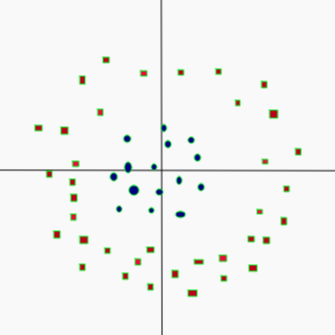
\includegraphics[scale=0.6]{../img/svc_non_linear} %https://medium.com/@george.drakos62/support-vector-machine-vs-logistic-regression-94cc2975433f
	\caption{Dati non divisibili in modo semplice}
	\label{fig:svc_non_linear}
\end{figure}

Tramite una funzione kernel trasformiamo questi due punti definiti dalle coordinate x e y, in punti avente coordinate x, y e z. Così facendo possiamo rivedere il tutto in 3 dimensioni e tracciare un iperpiano che suddivide correttamente i punti nello spazio, per poi successivamente ridefinirlo secondo le due dimensioni iniziali di partenza.

Come esplicato in un articolo di towards data science, riporto l'esempio esplicativo.
%TODO: refrenzia il post(https://towardsdatascience.com/https-medium-com-pupalerushikesh-svm-f4b42800e989), riporto l'esempio esplicativo:

Presi dei punti in uno spazio bidimensionale, ci capita la situazione in cui questi non sono suddivisibili tramite una retta.

Aggiungiamo una terza dimensione z e definiamola come segue:
\[ z = x^2 + y^2 \]

Il risultato ottenuto è mostrato in figura \ref{fig:svc_on_z_axis}.

\begin{figure}[h!]
	\center
	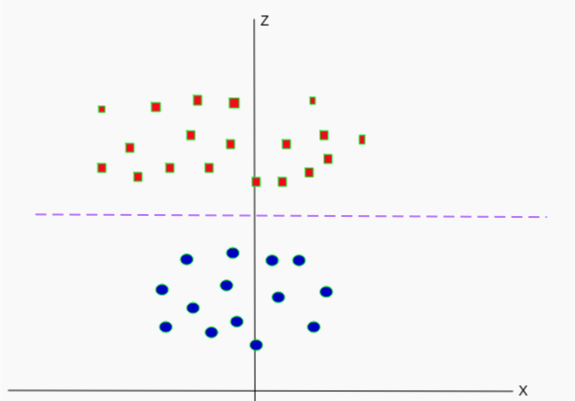
\includegraphics[scale=0.4]{../img/svc_on_z_axis} %https://medium.com/@george.drakos62/support-vector-machine-vs-logistic-regression-94cc2975433f
	\caption{Dati visti sull'asse z}
	\label{fig:svc_on_z_axis}
\end{figure}

Notiamo subito che ora è facile suddividere i punti in due distinti gruppi tramite una retta. Definiamo questa retta come:

\[ z = k \]

dove k è una costante. Dato che z è stato definito come:

\[ z = x^2 + y^2 \]

poniamo la retta k come segue:

\[ k = x^2 + y^2 \]

il che ci consente di ottenere una linea nello spazio a due dimensioni, che sarà esattamente la nostra divisione tra i gruppi.

Quindi quando ci si trova davanti a problemi n-dimensionali bisogna spesso ricorrere al trucco del kernel. Questo trucco prevede anche dei parametri $ C $ e $ \gamma $, detti iperparametri (o parametri di tuning).
Essi influiscono sulla selezione dell'iperpiano che si va ad ottenere nello spazio inziale:
\begin{itemize}
	\item $C$: è il parametro che consente di definire un costo nell'errore della suddivisione dei punti, vale a dire che nel caso in cui si scelga una C grande, ogni singolo errore avrà un costo elevato, andando cosi ad adattare il modello SVM nel modo più preciso possibile al training set. Adattando il modello in maniera eccessiva al training set, però, si rischierebbe di andare in overfitting e quindi comporterebbe ad una classificazione errata nel caso di esempi estranei all'insieme dei dati di allenamento. Avendo invece, una C piccola, il costo di errore sarà basso, il quale comporterà che durante l'allenamento del modello, saranno presenti diversi errori di classificazione, però, così facendo si sta generalizzando maggiormente il modello a nuovi casi da etichettare, il che può essere positivo. Vi rimando alla figura \ref{fig:tradeoff_img} che denota un buon livello di accuratezza, il quale sta a metà tra overfitting e underfitting.
	
	\item $\gamma$: questo parametro definisce fino a che punto arriva l'influenza di un singolo esempio di allenamento. Se ha ha un valore molto elevato, allora il limite della decisione dipenderà solo dai punti molto vicini alla linea, il che si traduce effettivamente nell'ignorare alcuni dei punti che sono molto lontani dal limite della decisione. Questo perché i punti più vicini ottengono più peso e si traduce in una curva ondulata come mostrato nel grafico precedente. D'altra parte, se il valore gamma è basso anche i punti più lontani ottengono un peso considerevole e otteniamo una curva più lineare.
\end{itemize}


\pagebreak

\subsubsection{Alberi di decisione}

Gli alberi di decisione (o decision trees), è un algoritmo di classificazione e regressione, che, fondamentalmente, basa la sua logica sull'apprendimento di una struttura, sulla domanda 'se questo allora...'/'altrimenti questo...' fino ad arrivare ad una decisione finale.

Prendo spunto da un esempio fatto nel libro 'Introduction to machine learning' in cui si vuole distinguere un animale tra: falco, pinguino, delfino, orso.
L'algoritmo lavora andando a fare determinate domande a cui puoi rispondere vero o falso. Si parte da una domanda che può semplicemente essere: "Ha le piume?". In questo modo si aprono due strade, "ha le piume" e "non ha le piume", suddividendo in due gruppi distinti gli animali. Prendendo quelli che non hanno le piume (orso e delfino), e facendo un'ulteriore domanda, che differenzia i due animali, si può arrivare a capire di quale animale si sta parlando. Seguendo quindi la domanda, "Ha le pinne?", possiamo capire che se la risposta è si, è il delfino, ovvero l'unico animale tra i 4 che non ha le piume e ha le pinne.

Seguendo questa logica è possibile arrivare - con le giuste domande - a fare delle predizioni.

Questo era un semplice esempio che non rispecchia la realtà, e i campi di utilizzo di questo algoritmo. Spesso i dati che vengono analizzati hanno dei valori di tipo continuo, quindi la domanda a cui si risponde, tendenzialmente, è del tipo: "x è maggiore di y?".

Impostando questa serie di domande il piano verrò diviso in diverse aree, ognuna delle quali è definita da una foglia dell'albero. 

\begin{figure}[h!]
	\center
	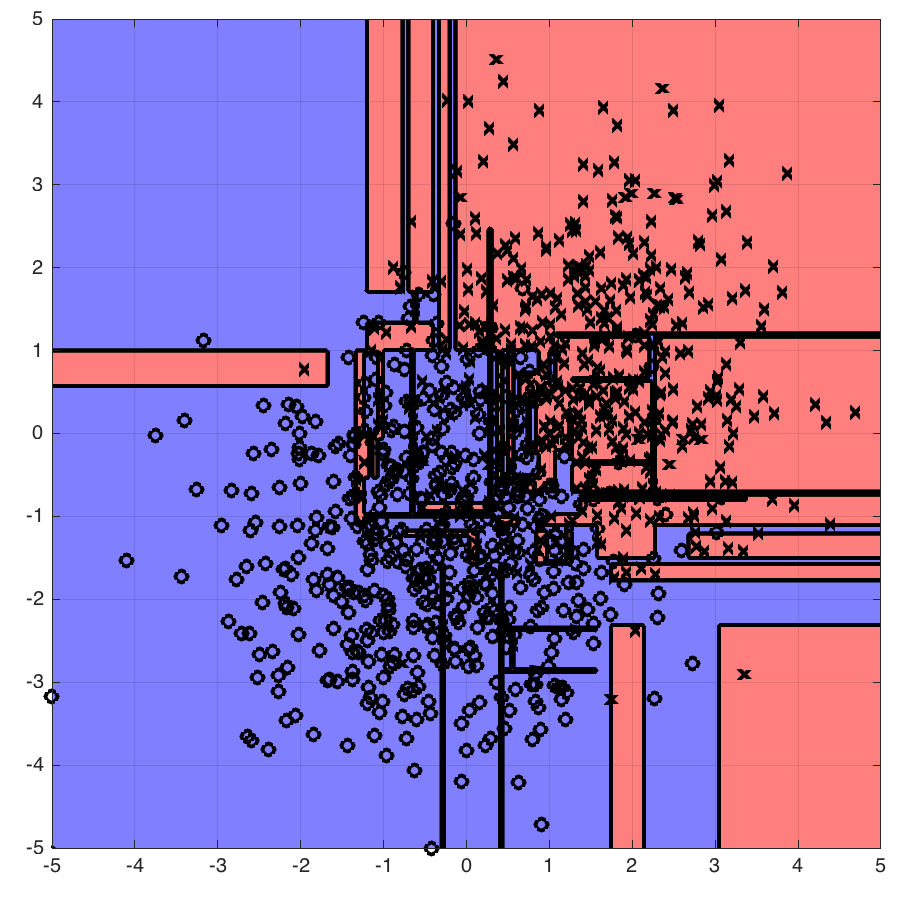
\includegraphics[scale=0.2]{../img/overfit_decision_trees1} %https://medium.com/@george.drakos62/support-vector-machine-vs-logistic-regression-94cc2975433f
	\caption{Overfitting dei dati con l'albero di decisione}
	\label{fig:overfit_decision_trees1}
\end{figure}

Come abbiamo già visto anche negli altri algoritmi, il problema dell'overfitting e underfitting è un problema ricorrente e nel caso dell'albero di decisione non è da meno.
Infatti se viene costruito un albero troppo dettagliato e quindi con un livello di profondità eccessivo si va ad adattare in maniera eccessiva (quindi in overfitting) al training set. 

In figura \ref{fig:overfit_decision_trees1} è raffigurato un albero di decisione dove è possibile notare zone blu e rosse eccessivamente piccole le quali sono sintomo di un eccessiva precisione nelle domande (quindi overfitting).

Analizzando un caso simile è possibile vedere tramite il grafico riportato in figura \ref{fig:overfit_decision_trees2} come l'errore su un test set (quindi un insieme di dati utile a testare il modello allenato), cresca con l'aumentare della profondità. Questo succede proprio perchè il modello non è generalizzato, ma si è allenato specificandosi in maniera eccessiva al training set.

\begin{figure}[h!]
	\center
	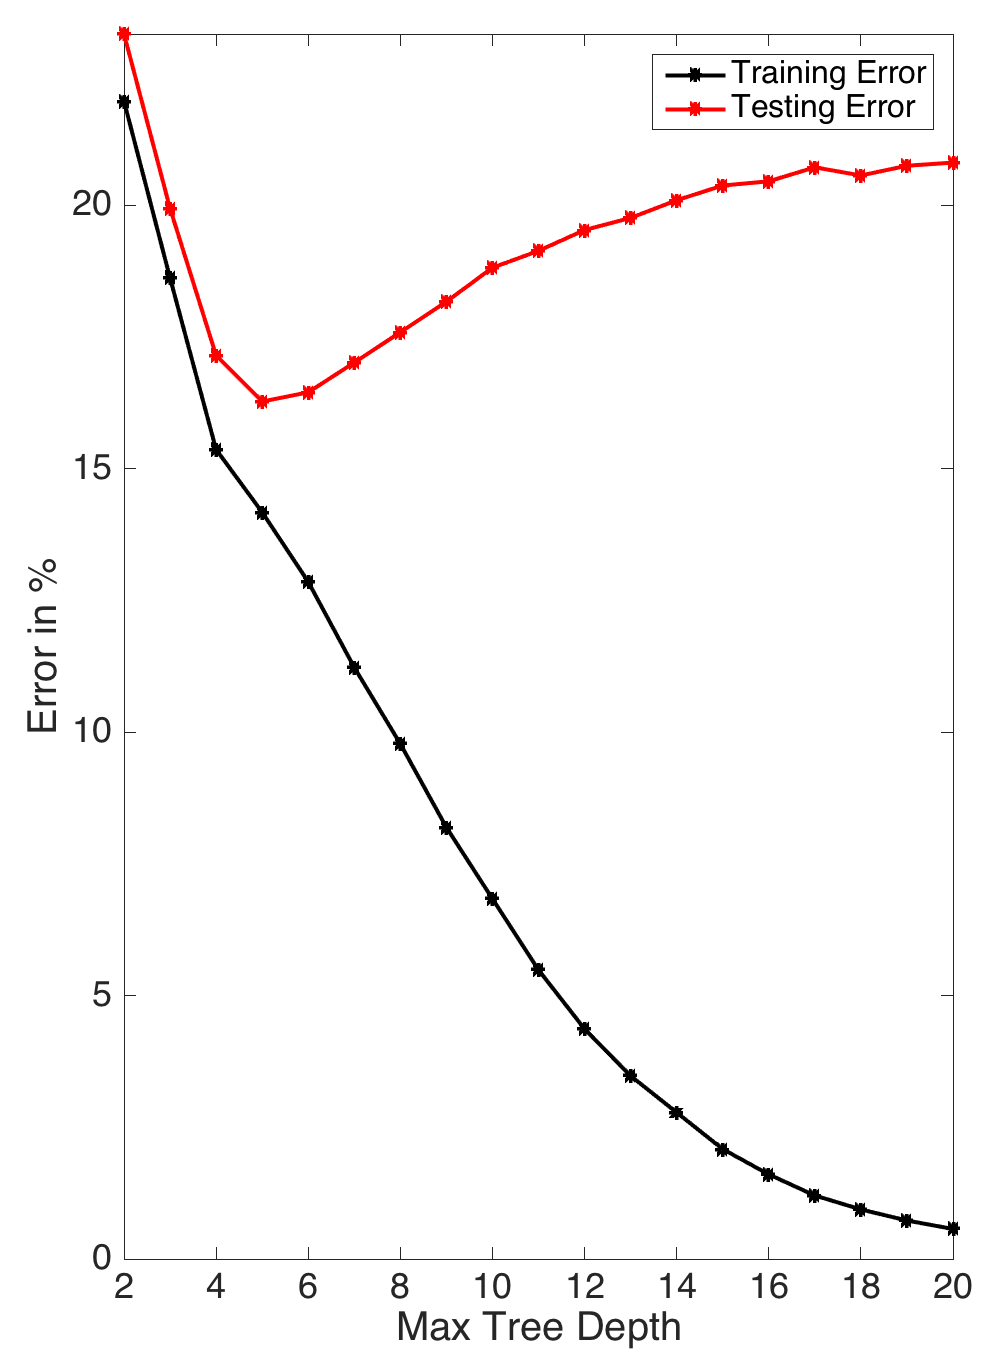
\includegraphics[scale=0.18]{../img/overfit_decision_trees2} %https://medium.com/@george.drakos62/support-vector-machine-vs-logistic-regression-94cc2975433f
	\caption{Grafico di overfitting con l'albero di decisione}
	\label{fig:overfit_decision_trees2}
\end{figure}

Per risolvere questo problema, esistono due strategie:
\begin{itemize}
	\item far terminare lo sviluppo dell'albero dopo pochi passi (pre-potatura): limitare la profondità dell'albero definendo una variabile che tenga conto della prodfondità dell'albero, la quale quando supera una soglia prefissata, interrompe lo sviluppo di questo
	
	\item rimuovendo i nodi che hanno contengono informazioni ridotte (post-potatura)
\end{itemize}

\pagebreak
\subsection{Unsupervised}
La tecnica "unsupervised" è il secondo importante approccio all'applicazione del machine learning. Esso consiste nella tecnica non supervisionata. Cosa si intende dire con non supervisionata? Come può una macchina imparare se nessuno la guida nella scelta di decisioni?
Questa è proprio la sfida che si vuole superare con questa tecnica, ovvero far estrapolare al calcolatore, delle informazioni "nascoste" all'interno dei dati che gli vengono forniti. Queste informazioni solitamente sono dei legami, schemi o regole che i dati tendono a seguire.

Ci sono diversi utilizzi di machine learning non supervisionato, in questa sezione ci limiteremo a elencarne alcuni.

Il principale algoritmo di unsupervised learning è il clustering, ossia un algoritmo in grado di suddividere in gruppi distinti, degli elementi che hanno dati e caratteristiche in comune. Per essere più chiari, vediamo subito un possibile esempio.

Supponiamo di aver scattato una serie di foto i cui soggetti sono delle persone, magari nostri amici o parenti e decidiamo di caricarle su un social network. Durante il caricamento, il social su cui le stiamo caricando, si permette di visionare le foto e applicare proprio un algoritmo di clustering. In che modo? L'algoritmo non sa nè chi siano le persone raffigurate nè quante esse siano. L'algoritmo andrà a cercare tutti i volti nelle foto che abbiamo caricato e successivamente, dopo aver ottenuto una lista di tutti i volti estrapolati da ogni foto, tramite un algoritmo di clustering va a cercare somiglianze in questi volti, andando così a raggruppare le foto dove è presente lo stesso soggetto.

Un altro esempio di utilizzo ricade nella sicurezza informatica. Al giorno d'oggi i tipi di attacchi conosciuti sono probabilmente solo la punta dell'iceberg. Ricorrendo però a tecniche come questa possiamo riuscire ad bloccare anche attacchi tuttora sconosciuti. 
Supponiamo di essere loggati nel nostro sito bancario. Tramite il machine learning unsupervised il sistema andrà a memorizzare tutte le nostre operazioni per la nostra sicurezza. Supponiamo di effettuare quotidianamente delle specifiche operazioni ad un fissato orario, in una specifica località geografica. Bene, queste informazioni vengono salvate dal calcolatore il quale le utilizzerà per creare dei cluster, ossia riconoscere quali sono le nostre operazioni comuni, riconoscendole tramite, orario, località geografica e altre possibili informazioni. A questo punto supponiamo che un malintenzionato dall'altra parte del mondo, ad un orario differente dal nostro orario abituale, entri nel nostro profilo bancario.   L'algoritmo sarebbe in grado di notare che è in atto qualcosa di strano. Questo, perchè tramite il clustering, nessuno gli deve dire quali sono le operazioni comuni fatte dall'utente, bensì, il computer stesso, è in grado di riconoscerle e mandare un messaggio di allarme se individua dei possibili outlier. 


\pagebreak
\subsection{Semi-supervised}

L'approccio semi-supervised, non è un vero e proprio approccio, bensì una tecnica che sta a metà tra le due appena viste (supervisionato e non supervisionato). Questa tecnica consiste nel combinare le due tecniche e fornire un risultato basandosi su un input eterogeneo: etichettato e non.

Questo approccio risulta utile quando si ha una grande mole di dati, e gli utenti che sono in grado di etichettare i dati sono utenti specializzati. Nella situazione reale, non sempre questo è possibile, proprio perché possono mancare risorse umane competenti o tempistiche adeguate per classificare tutti i dati.

Esistono differenti algoritmi per l'apprendimento automatico mediante un sistema semi-supervisionato:
\begin{itemize}
	\item Self training
	\item Multi-view training
	\item Self-ensembling
\end{itemize}

Per quanto riguarda il multi-view training, esso mira a formare diversi modelli con diverse visualizzazioni dei dati. Idealmente, queste viste sono complementari e i modelli possono collaborare per migliorare il risultato finale. Queste viste possono differire in diversi modi, ad esempio nelle funzionalità che utilizzano, nelle architetture dei modelli o nei dati su cui i modelli vengono formati.

Il self-ensembling, come il multi-view training, punta a combinare diverse varianti dei modelli. A differenza però di quest'ultimo, la diversità nei modelli non è un punto chiave perchè il self-ensembling utilizza principalmente un singolo modello in diverse configurazioni al fine di rendere più affidabili le previsioni del modello. 

A titolo di esempio vediamo più in dettaglio l'algoritmo di Self training che è stato uno dei primi ad essere sviluppato ed è l'esempio più diretto di come le previsioni di un modello possono essere incorporate nel training del modello.

L'algoritmo di auto-allenamento prevede quindi di basarsi per quanto può su dei dati che sono stati preventivamente definiti secondo un particolare modo e altri che sono solamente dei dati da analizzare. Questi ultimi vengono comunque utilizzati, ma in maniera più cauta, ovvero, prima di allenare il modello per imparare a fare una predizioni, il modello si concentrerà ad etichettare gli input che ancora sono senza alcuna etichetta.

Come viene spiegato in un articolo su ruder.io %[https://ruder.io/semi-supervised/index.html\#relatedmethodsandareas], 
la logica di classificazione dei dati non ancora classificati segue quanto scritto:		\\
"Formalmente, l'auto etichettamento avviene su un modello M avente un training set etichetto L con delle etichette contenute in C e un set non etichettato U. Ad ogni iterazione, per ogni x in U, il modello fornisce delle predizioni su m(x) sottoforma di probabilità p(x, c) ovvero probabilità che x appartenga alla classe c per ogni c in C. Tra le probabilità appena calcolate, definiamo P(x, c) come la probabilità avente il valore maggiore, allora se P è più grande di una soglia T, x verrà aggiunto a L con l'etichetta c. Questo processo viene ripetuto per un numero fisso di iterazioni o fino a quando non ci sono più dati da etichettare.".[nota: traduzione libera del testo: nell'originale è presente una formula ceh io rendo a parole]

Di seguito vediamo uno pseduo-codice che segue quanto detto sopra:

\begin{algorithmic}[1]
	\Repeat
	\State $m \gets train\_model(L)$
	\For {$x \in U$}
	\If {$\max m(x) > \tau$}
	\State $L \gets L \cup \{(x, p(x))\}$
	\EndIf
	\EndFor
	\Until {no more predictions are confident}
\end{algorithmic}

\pagebreak
\subsection{Reinforcement learning}
Il quarto ed ultimo approccio chiamato Reinforcement learning, è un approccio che si differenzia da quelli visti fino ad ora. Questo paradigma si occupa di problemi di decisioni sequenziali, in cui l'azione da compiere dipende dallo stato attuale del sistema e ne determina quello futuro. In altre parole, questo è un sistema dinamico che può apprendere in seguito ad ogni decisione presa, a prescindere che questa sia giusta o sbagliata.

\begin{figure}[h!]
	\noindent
	\center
	\label{fig:rl_scenario}
	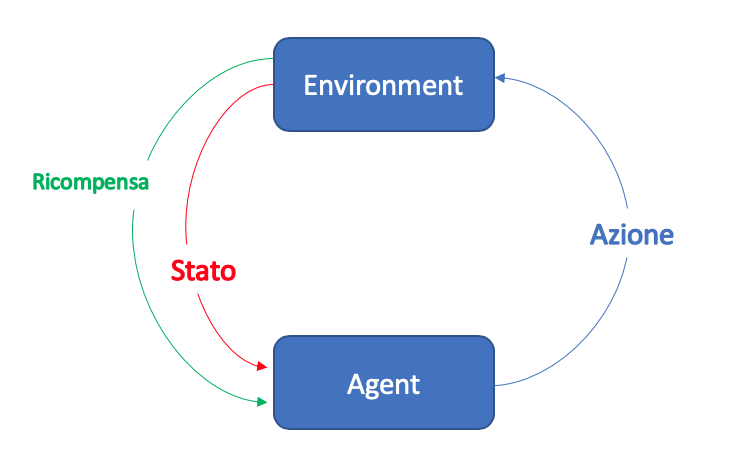
\includegraphics[scale=0.5]{../img/rl_scenario}
	\caption{Scenario RL}
\end{figure}
% (https://www.aitrends.com/education/udacitys-school-of-ai-opens-the-new-deep-reinforcement-learning-nanodegree-program-for-enrollment/) (https://www.guru99.com/reinforcement-learning-tutorial.html)

Quando il sistema prende una decisione, esso otterrà una "ricompensa" che può essere un punteggio, che sarà alto o basso a seconda se la decisione presa è giusta o sbagliata. Con questa logica, la macchina cercherà di fare sempre meglio per arrivare a ottenere il punteggio più alto possibile, prendendo così solo le decisioni corrette. 

Di seguito, sono citati dei casi di utilizzo di questo approccio:

\begin{itemize}
	\item Imparare a giocare a scacchi
	\item Imparare a guidare un veicolo
\end{itemize}

\pagebreak
\section{Ridimensionamento delle funzionalità}

    Nel machine learning, come abbiamo visto, l'input, gioca un ruolo fondamentale nello sviluppo di un modello, che riesca a predire nel modo corretto i nuovi dati che verrano esaminati da quest'ultimo.
In questo testo ci concentreremo proprio sul riconoscimento dei volti all'interno delle immagini, quindi per per parlare dell'importanza del ridimensionamento delle feature, faremo riferimento proprio all'analisi di immagini che raffigurano persone, animali o oggetti.

Spesso, ci troviamo davanti a dei dati di dimensioni eccessive, i quali comportano in primis dei problemi a livello tempistico e anche a problemi a livello computativo.

Ci basti pensare che quando si cerca di analizzare un'immagine per estrapolarne delle informazioni (riconoscimento di oggetti, persone, animali) dobbiamo prendere passare in rassegna tutti i pixel! Supponiamo di prendere anche un'immagine, a bassa risoluzione, ad esempio 500x500, significherebbe trovarsi davanti a $ 500^2 $ pixel, ovvero 250.000 elementi per una singola immagine! Questo comporterebbe quindi, di analizzare uno spazio sovra dimensionato, con, appunto 250.000 dimensioni.

Pensare ad uno spazio di quelle dimensioni è impensabile, proprio per questo ci vengono in soccorso delle tecniche che si occupano di ridurre il numero di elementi che definsicono l'oggetto, senza perdere, o meglio, estrapolando, solamente le informazioni più utili che permettono di differenziare un oggetto da un'altro.

Pensiamo ad esempio a un'immagine in cui è raffigurato il volto di una persona. E' normale pensare che non tutti i pixel siano di fondamentale importanza per riconoscere il soggetto raffigurato. Ad esempio, tutti i pixel presenti nei bordi dell'immagine saranno sicuramente da scartare in quanto non ci diranno niente sulla persona raffigurata, così come molti altri pixel che raffigurano parti poco interessanti, ad esempio lo sfondo dell'immagine. Vediamo nel dettaglio quali sono gli strumenti più utilizzati per risolvere questo tipo di problemi.


\subsection{PCA (Principal Component Analysis)}
PCA (Principal Component Analysis) è un metodo di riduzione delle dimensionalità. Lo scopo di PCA è quindi quello di diminuire il numero di variabili, limitando il più possibile la perdita di informazioni. 

In primo luogo, viene calcolata la media per ogni feature. Una volta calcolata, il vettore risultante lo faremo coincidere con l'origine degli assi, in questo modo ogni punto verrà traslato di conseguenza. A questo punto viene calcolata la retta che meglio si adatta a tutti i punti, ovvero la retta R che minimizza la somma delle distanze dei punti da R. Questa viene chiamata $ PC_{1} $. Si ripete questo passaggio per ogni dimensione, mantenendo la perpendicolarità della nuova retta (o $ PC_{n} $) rispetto all'ultima retta calcolata (o $ PC_{n-1} $). 
Una volta calcolate tutte i principal component dello spazio PCA si va a calcolare, per ognuna di esse, l'autovettore, il quale sarà utilizzato per determinare la nuova posizione di ogni punto scalandolo sul rispettivo asse. Una volta scalati tutti i punti si può calcolare la varianza per ogni asse. Il valore della varianza $\sigma$ rispetto al $ PC $ x, calcolata in percentuale, ci dice quanto pesa l'informazione contenuta su quell'asse. Questo ci permetterà quindi, di eliminare gli assi meno interessanti, ovvero gli assi con la varianza più bassa. 

Questa tecnica, oltre a semplificare il lavoro di manipolazione delle caratteristiche, aiuta a migliorare i risultati dell'algoritmo di machine learning. PCA aiuta gli algoritmi di machine learning perché estrapola le informazioni realmente utili per predire la classe o il valore da attribuire ad un oggetto. Tutte le informazioni di contorno, come ad esempio, i pixel situati sul bordo di un'immagine possono essere fuorvianti per l'algoritmo di apprendimento. Questo è il motivo per cui esso semplifica e ottimizza i valori risultanti.

PCA vede un vasto utilizzo nell'ambito di:
\begin{itemize}
	\item riconoscimento facciale
	\item image compression
	\item rilevamento di pattern in campi ad alta dimensionalità
	\item data mining
\end{itemize}

\pagebreak

\subsection{t-SNE (t-distributed stochastic neighbor embedding)}
%Documenta con delle immagini prendedole dal video https://www.youtube.com/watch?v=NEaUSP4YerM
t-SNE è una tecnica di riduzione della dimensionalità non lineare che si presta particolarmente alla mappatura di spazi ad alta dimensionalità in uno spazio a due o tre dimensioni, nel quale possono essere visualizzati tramite un grafico di dispersione. L'algoritmo modella i punti in modo che oggetti vicini nello spazio originale risultino vicini nello spazio a dimensionalità ridotta, e oggetti lontani risultino lontani.

Per spiegare il funzionamento di questo algoritmo, basiamoci su un caso semplice: un set $S$ di dati bidimensionale. Con questo esempio spiegheremo quindi il funzionamento di t-SNE e come è possibile passare da due dimensioni, ad una sola, mantenendo le corrette distanze. Per farlo ci baseremo sulle probabilità che un elemento sia vicino ad un'altro. Quindi per ogni punto x, andiamo a centrare su di esso una curva gaussiana. Per ogni altro punto $ y $  tale che:
\[ y \in S / x \]
andiamo a inserirlo sotto la distribuzione gaussiana, per poi calcolarne la probabilità di densità (o score).
%la quale verrà utilizzata per calcolare la probabilità che ogni altro elemento, sia vicino a x. 

Viene utilizzata la curva gaussiana perchè lavora bene su casi come questo: restituisce un'alta probabilità se un elemento è molto vicino e una molto bassa probabilità se questo è lontano. A questo punto normalizziamo la curva per tutti i punti in modo che essi abbiano una misura proporzionata e non indipendente. La distribuzione può in realtà essere manipolata tramite una variabile chiamata perplessità, la quale va a modificare la varianza e quindi l'ampiezza della curva.
A questo punto avremo ottenuto la matrice $ M_{1} $ quadrata con tutti gli score per ogni coppia. Ora andiamo a inserire tutti i punti, in maniera casuale su un'unico asse. Analogamente a quanto appena fatto, calcoliamo la probabilità di vicinanza tra i punti, con la differenza che questa volta useremo la distribuzione di Student (in inglese t-distribution, da cui deriva la t di t-SNE). Analogamente, otterremo una seconda matrice $ M_{2} $ quadrata, la quale sarà, probabilmente, molto diversa da $ M_{1} $. L'obiettivo adesso, sarà quello di adattare la matrice $ M_{2} $ a $ M_{1} $. Così facendo riusciremo a mantenere i cluster visualizzabili nel grafico bidimensionale.

Nella seconda parte dell'algoritmo, viene usata una t-distribution perchè distacca meglio i cluster nel piano generato. Se avessimo usato una distribuzione gaussiana, come nella prima parte, il risultato ottenuto sarebbe stato meno visibile, in quanto tutti i cluster si sarebbero ammassati al centro.

Questo è un esempio piuttosto semplice, ma nella realtà si possono adattare spazi a $n$ dimensioni con $ n \gg 2 $. Nel Capitolo 3 lo utilizzeremo per ridurre le dimensioni da uno spazio molto vasto, ad uno spazio bidimensionale o al più a 5 dimensioni. Vedremo quindi, utilizzando questo algoritmo, quali sono le prestazioni che riesce a fornire nel caso del riconoscimento facciale e di classificazione dei soggetti.
% 
%			CAPITOLO 2: Stato dell'arte
% 


% Pagina dichiusura del LIM


\end{document}


 
